
\subsection{Chapter 2}

\begin{p}%{55}
{Given a manifold $M$, define charts for $TM$ starting from charts $\varphi_\alpha:U_\alpha\rightarrow \R^n$ as follows. Let $V_\alpha$ be the subset of $TM$ given by $V_\alpha=\{v\in TM:\pi(v)\in U_\alpha\}$. Show that every point in $TM$ lies in some set $V_\alpha$. Define
maps $\psi_\alpha:V_\alpha\rightarrow \R^n\times \R^n$ by $\psi_\alpha(v)=(\varphi_\alpha(\pi(v)),(\varphi_\alpha)_*v)$, where we think of $(\varphi_\alpha)_*v$, which is really a tangent vector to $\R^n$, as
a vector in $\R^n$. Give $TM$ the topology in which open sets are the unions of sets of the form $O\subset V_\alpha$ such that $\psi_\alpha(O)\subset \R^n\times \R^n$ is open. Check that $\psi_\alpha$ are charts, so that $TM$ is a manifold. Check that $\pi:TM\rightarrow M$ is smooth.}
\end{p}
{Every point $v$ in $TM$ is in some $V_\alpha$ since $v$ is the tangent vector at some point $p$ (as given by $p=\pi(v)$), and every point $p$ is in some set $U_\alpha$. To establish that $\psi_\alpha$ are charts and $TM$ is a smooth manifold, note that $\varphi_\alpha$ is smooth and so is the pushforward, so $\psi_\alpha$ is smooth, too. Transition functions
from one chart to another are likewise smooth, since these are compositions of smooth $\psi_\alpha$ and $\psi^{-1}_\beta$ which overlap on some open set. The projection $\pi$ is smooth because we can define 
the $\R^{2n}\rightarrow \R^n$ version of the map by just ignoring the last $n$ coordinates. But this map is just $\varphi_\alpha\circ\pi\circ\psi_\alpha^{-1}$, so $\pi$ must be smooth.}

\begin{p}%{56}
{Given bundles $\pi:E\rightarrow M$ and $\pi':E'\rightarrow M'$, show that the maps $\psi:E\rightarrow E'$ and $\phi:M\rightarrow M'$ are a bundle morphism iff $\pi'\circ\psi=\phi\circ\pi$. Show that
$\psi$ uniquely determines $\phi$.}
\end{p}
{Bundle morphisms respect the bundle structure, i.e.~the split into fiber and base. If $\pi'\circ\psi=\phi\circ\pi$, then the fiber in $E$ over $p$ must be mapped to the fiber in $E'$ over $p'=\phi(p)$, or else the relationship would not hold. Conversely, if the fibers are mapped to the appropriate base
points, then it doesn't matter if we do the tangent space map first or second.}

\begin{p}%{57}
{Check that $\phi_*$ is smooth when we make the tangent bundle into a manifold as in the previous exercise.}
\end{p}
{(typo on the ``previous'' exercise?) A map between two manifolds is smooth if it takes smooth functions on the first manifold to smooth functions on the second. Points in the manifold in 
question are vectors $v$, so functions of them are 1-forms $\om$. Using an exact 1-form $df$ we have
$df(v)=v(f)$. When $v=\phi_*(u)$ we get $df(\phi_*(u))=\phi_*(u)(f)=u(\phi^*f))=u(f\circ\phi)$, which is 
smooth.}

\begin{p}%{58}
{Show that if $\phi:M\rightarrow M'$ is a diffeomorphism, then $\phi_*:TM\rightarrow TM'$ is a bundle isomorphism.}
\end{p}
{When $\phi$ is an isomorphism, the tangent spaces $T_pM$ and $T_\phi(p)M'$ are 
isomorphic, since the smooth functions on $M$ get mapped isomorphically to smooth functions on $M'$. Since
the pushforward is smooth and linear, it's an isomorphism of the tangent spaces.}

\begin{p}%{59}
{Show that for any manifold $M$, the tangent bundle $\pi:TM\rightarrow M$ is locally trivial.}
\end{p}
{The induced charts $\psi_\alpha$ give us a trivialization, with $\R^n$ as the standard fiber.}

\begin{p}%{60}
{Describe a bundle that is not locally trivial.}
\end{p}
{}

\begin{p}%{61}
{Check that the tangent bundle of a manifold is a vector bundle.}
\end{p}
{To be a vector bundle, the 
local trivialization must be fiberwise linear. The standard fiber for a tangent bundle is $\R^n$, and the  
trivialization is linear because it is just the pushforward (exercise 17, part I).}

\begin{p}%{62}
{A 1-dimensional bundle is called a (real or complex) line bundle. Check that the M\"obius strip is a real line bundle if we regard the standard fiber as being $\R$.}
\end{p}
{Locally the M\"obius strip is just $\R^2$, so the trivialization is linear.}

\begin{p}%{63}
{Show that if a vector bundle morphism is a diffeomorphism, its inverse is a vector bundle morphism.}
\end{p}
{}

\begin{p}%{64}
{Show that a (smooth (typo?)) section of the tangent bundle is a vector field.}
\end{p}
{A section of the tangent bundle
assigns to each point in the base space vector in its tangent space. From this we obtain a 
vector field from the pointwise action of the tangent vectors. The output of the vector field is again a 
smooth function since the
section is smooth; the directional derivative (function value) changes smoothly from point to point since
the tangent vectors do.}

\begin{p}%{65}
{Show that $\Gamma(E)$ is a module over $C^\infty(M)$.}
\end{p}
{The first two conditions are defined 
in the text. The other two are simply: $(fg)s=f(gs)$ since $(fg)s:=((fg)s)(p)=(fg)(p)s(p)=f(p)g(p)s(p)=f(gs)(p)$ for
$f,g\in C^\infty (M)$. }

\begin{p}%{66}
{Show that every section of the M\"obius strip (viewed as a real line bundle over $S^1$) vanishes somewhere. Conclude that hte M\"obius strip hos no basis of sections, hence is not trivial.}
\end{p}
{can't cut the M\"obius strip and make a cylinder unless there's a zero somewhere.}

\begin{p}%{67}
{Show that the dual vector bundle really is a vector bundle. Also, show that given a basis
of section $e_i$ of a vector bundle $E$, there is a unique dual basis $e^i$ of sections of $E^*$ such that for each point $p\in M$, $e^i(p)$ is the basis of $E^*_p$ dual to the basis $e_i(p)$ of $E_p$.}
\end{p}
{The basic idea, I think, is that since $E|_U$ is locally equivalent to 
$U\times \mathbb{R}^n$ for any open set $U$, then since $E^*$ just replaces 
$E_p$ with $E^*_p$ everywhere, 
$E^*|_U$ must be locally equivalent to $U\times (\mathbb{R}^n)^*=U\times \mathbb{R}^n$. 
This makes $E^*$ a manifold. To see that it is a vector bundle, just use the canonical dual basis when 
mapping $E_p^*$ to $\mathbb{R}^n$. 
}

\begin{p}%{68}
{Show that if $s$ is a section of a vector bundle $E$ over $M$ and $\lambda$ is a 
section of $E^*$, there is a smooth function $\lambda(s)$ on $M$ given by 
\[\lambda(s)(p)=\lambda(p)(s(p))\] for all $p\in M$. Show that $\lambda(s)$ depends $C^\infty(M)$-linearly on $\lambda$ and $s$.}
\end{p}
{Locally, the vector bundles are trivial, so locally the section
looks like a function from $M$ to $V$ ($V^*$), where $E_p=\{p\}\times V$. We can then 
apply $\lambda$ to $s$ pointwise to obtain the function. It is smooth since the sections are smooth. 
$\lambda(s)$ is linear over $\lambda$ and $s$ since the action of the cotangent vector on the tangent vector is linear in each argument. We get the $C^\infty(M)$ part since the action is pointwise and smooth.}

\begin{p}%{69}
{Show that a section of the cotangent bundle is the same as a 1-form.}
\end{p}
{A 1-form is a
map taking vector fields to functions on the manifold. Interpreting vector fields as sections of
the tangent bundle, means that a 1-form is a map from sections of $TM$ to functions on $M$. By the
previous exercise we see that a section of $T^*M$ is just such a map, so a section of the cotangent
bundle is a 1-form.}

\setcounter{p}{76}

\begin{p}%{77}
{Show that the conditions $g_{\alpha\alpha}=1$ and $g_{\alpha\beta}g_{\beta\gamma}g_{\gamma\alpha}=1$ imply $g_{\beta\alpha}^{-1}=g_{\alpha\beta}$. Show that for any sequences $\alpha_1,\dots,\alpha_n$ and $\beta_1,\dots,\beta_m$ with $\alpha_1=\beta_1$ and $\alpha_n=\beta_m$, they 
imply $$g_{\alpha_1\alpha_2}\cdots g_{\alpha_{n-1}\alpha_n}=g_{\beta_1\beta_2}\cdots g_{\beta_{m-1}\beta_m}.$$
}
\end{p}
{Letting $\gamma=\alpha$ in the cocyle condition yields $g_{\alpha\beta}g_{\beta\alpha}g_{\alpha\alpha}=1$. Then using $g_{\alpha\alpha}=1$ we obtain
$g_{\alpha\beta}g_{\beta\alpha}=1$, so $g_{\beta\alpha}^{-1}=g_{\alpha\beta}$. Now
observe that $g_{\alpha_1\alpha_{n-1}}g_{\alpha_{n-1}\alpha_n}=g_{\alpha_1\alpha_n}$ since
multiplying by the inverse of the righthandside gives $g_{\alpha_1\alpha_{n-1}}g_{\alpha_{n-1}\alpha_n}g_{\alpha_n\alpha_1}=1$. By induction we can expand this expression to
$g_{\alpha_1\alpha_2}\cdots g_{\alpha_{n-1}\alpha_n}$. Similarly, we can start with
$g_{\beta_1\beta_{m-1}}g_{\alpha_{m-1}\beta_m}=g_{\alpha_1\alpha_n}$ and obtain $g_{\beta_1\beta_2}\cdots g_{\beta_{m-1}\beta_m}$, so they must be equal.}


\newpage
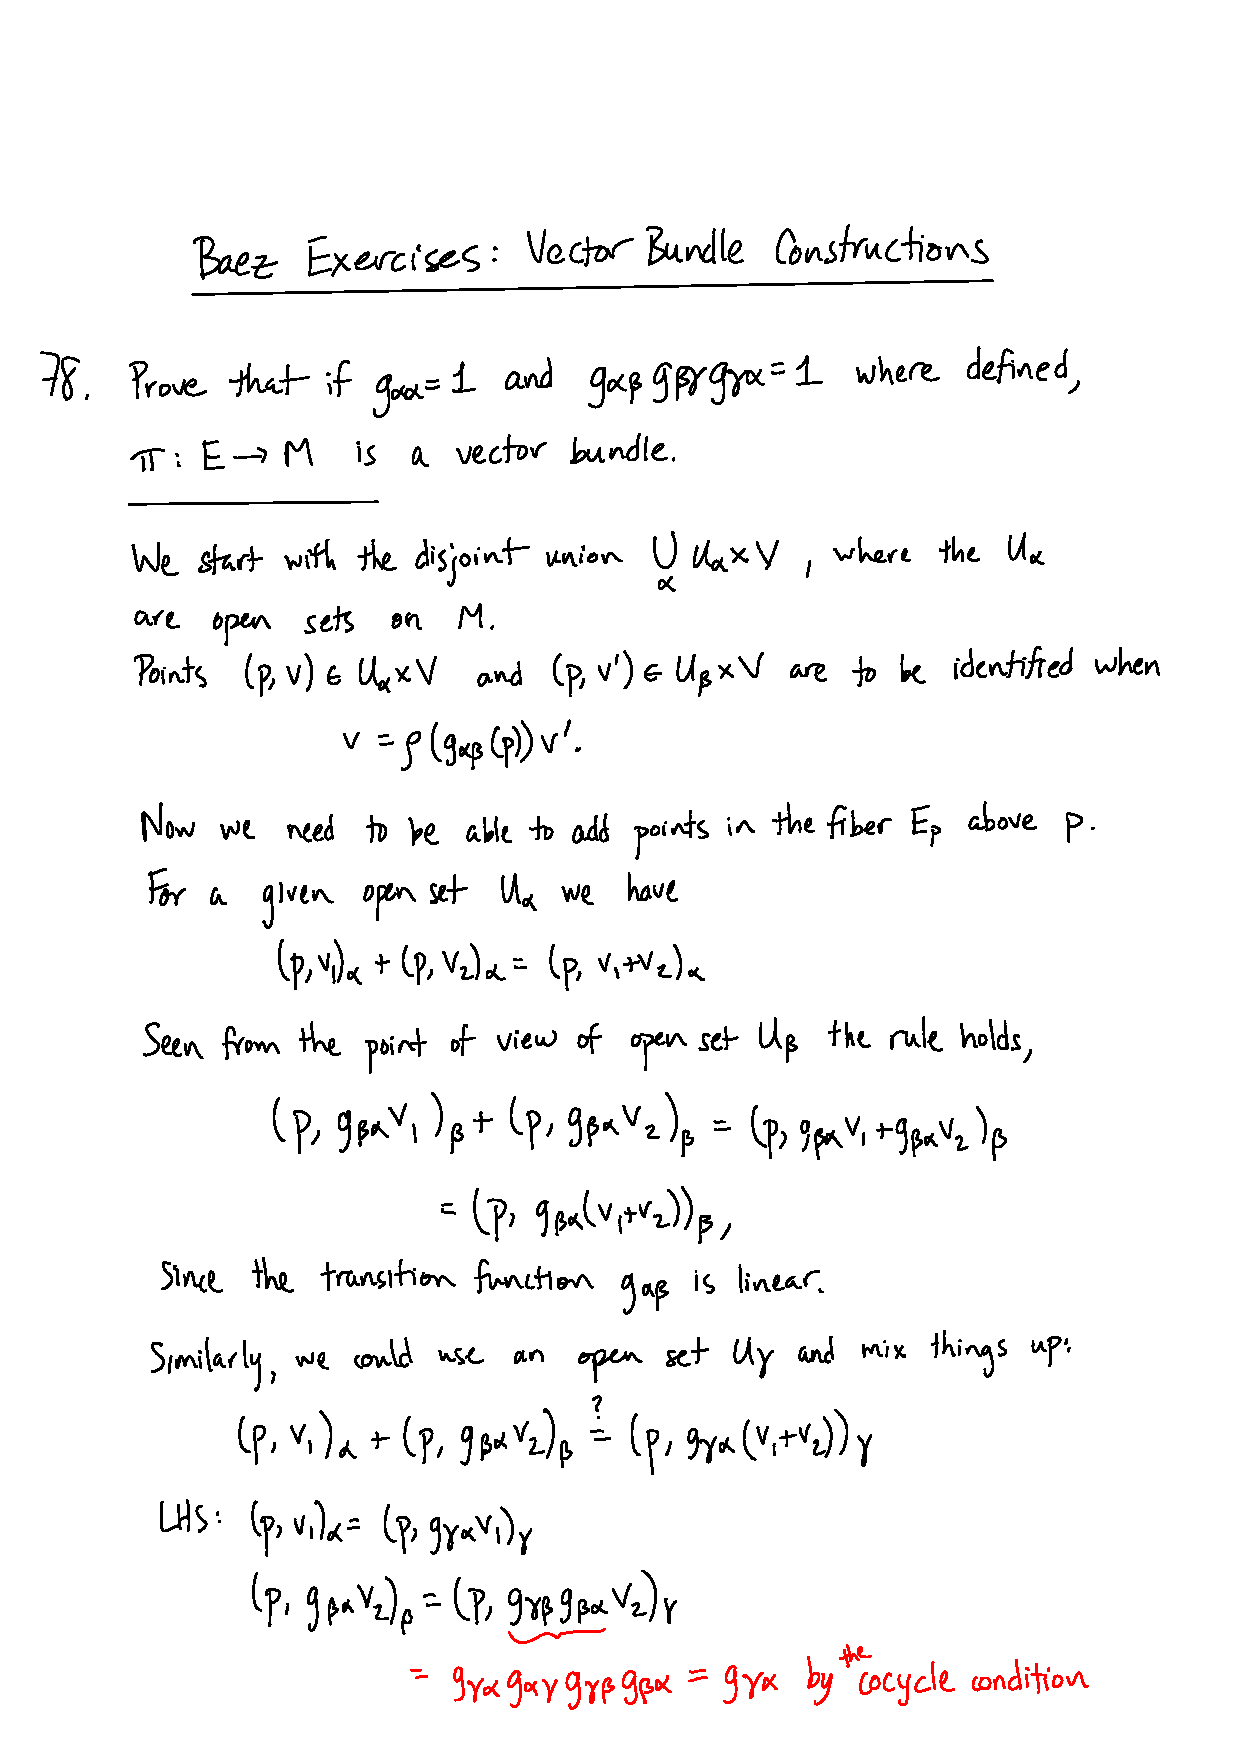
\includepdf[pages=-]{src/gfkg223.pdf}
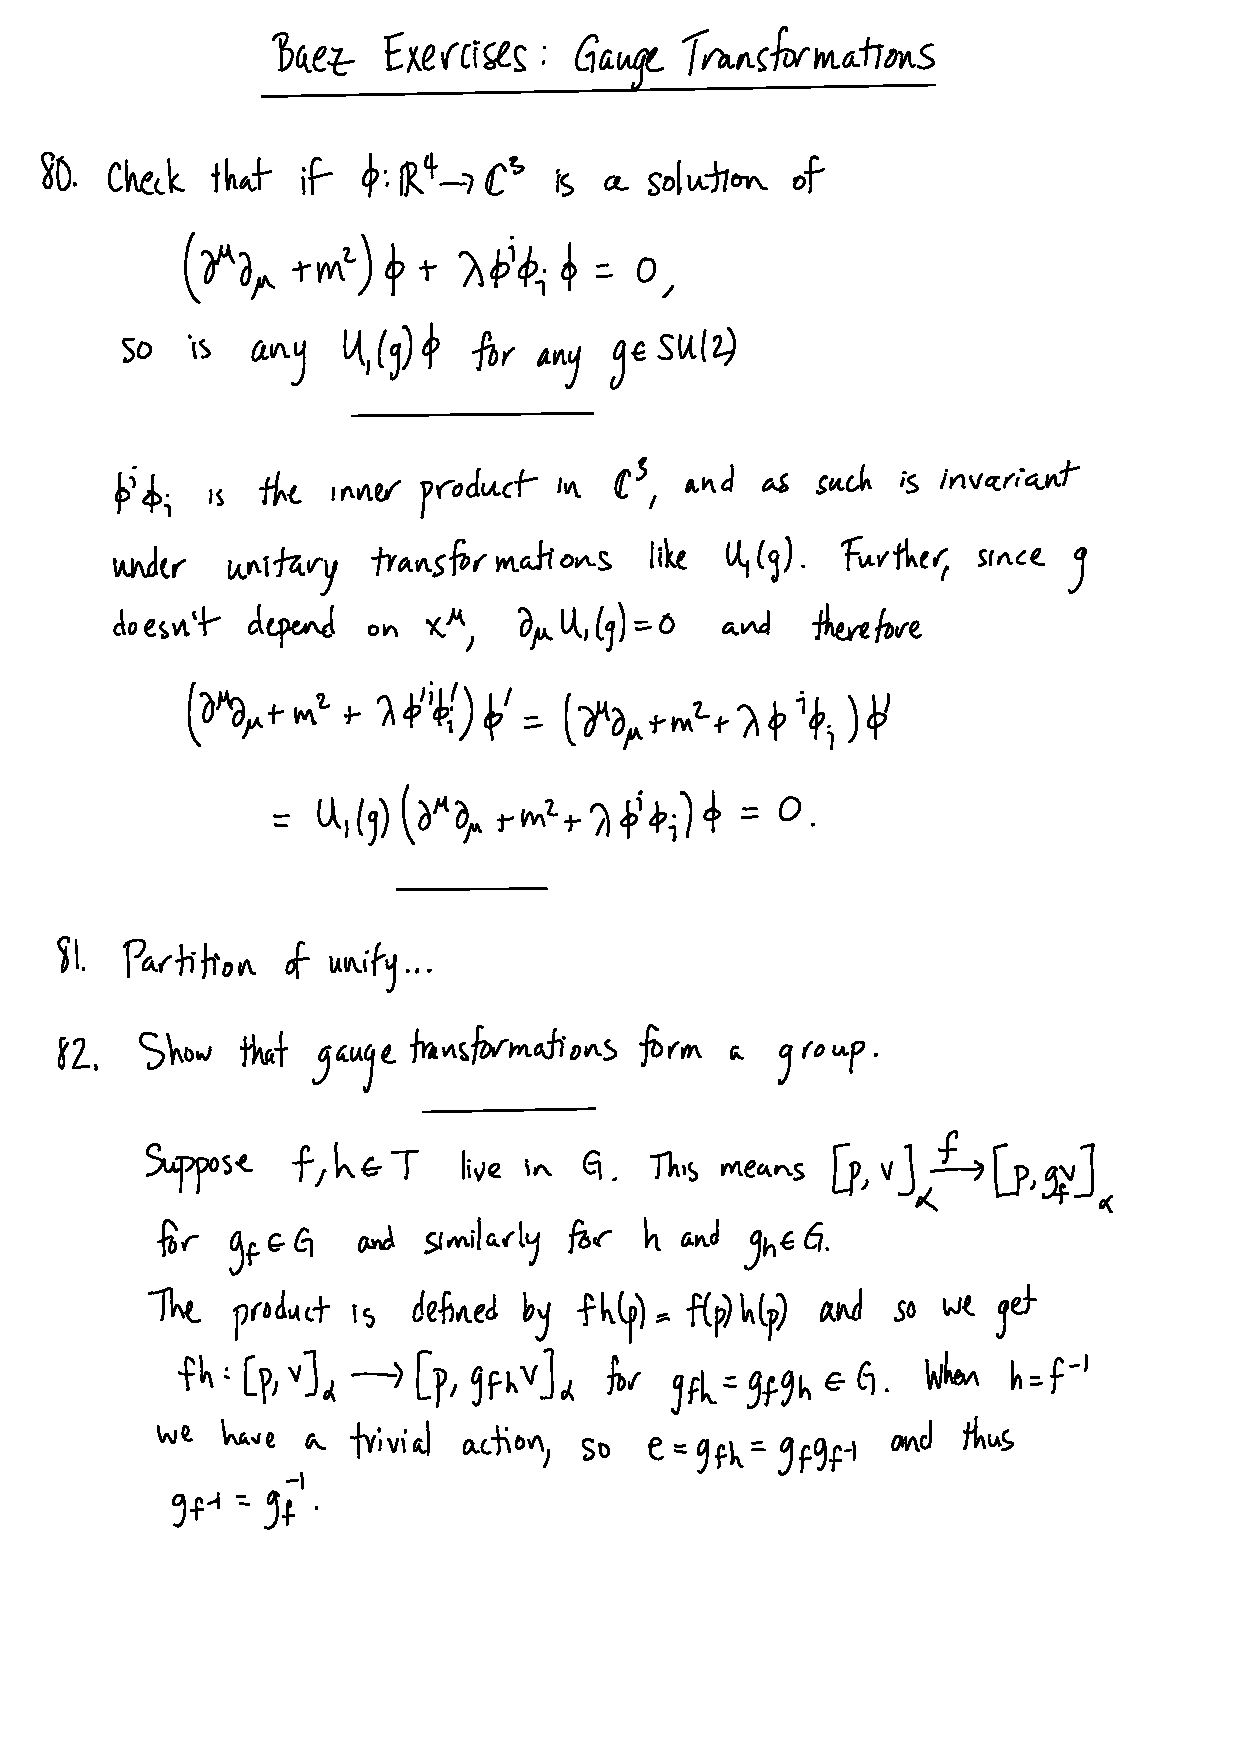
\includepdf[pages=-]{src/gfkg224.pdf}
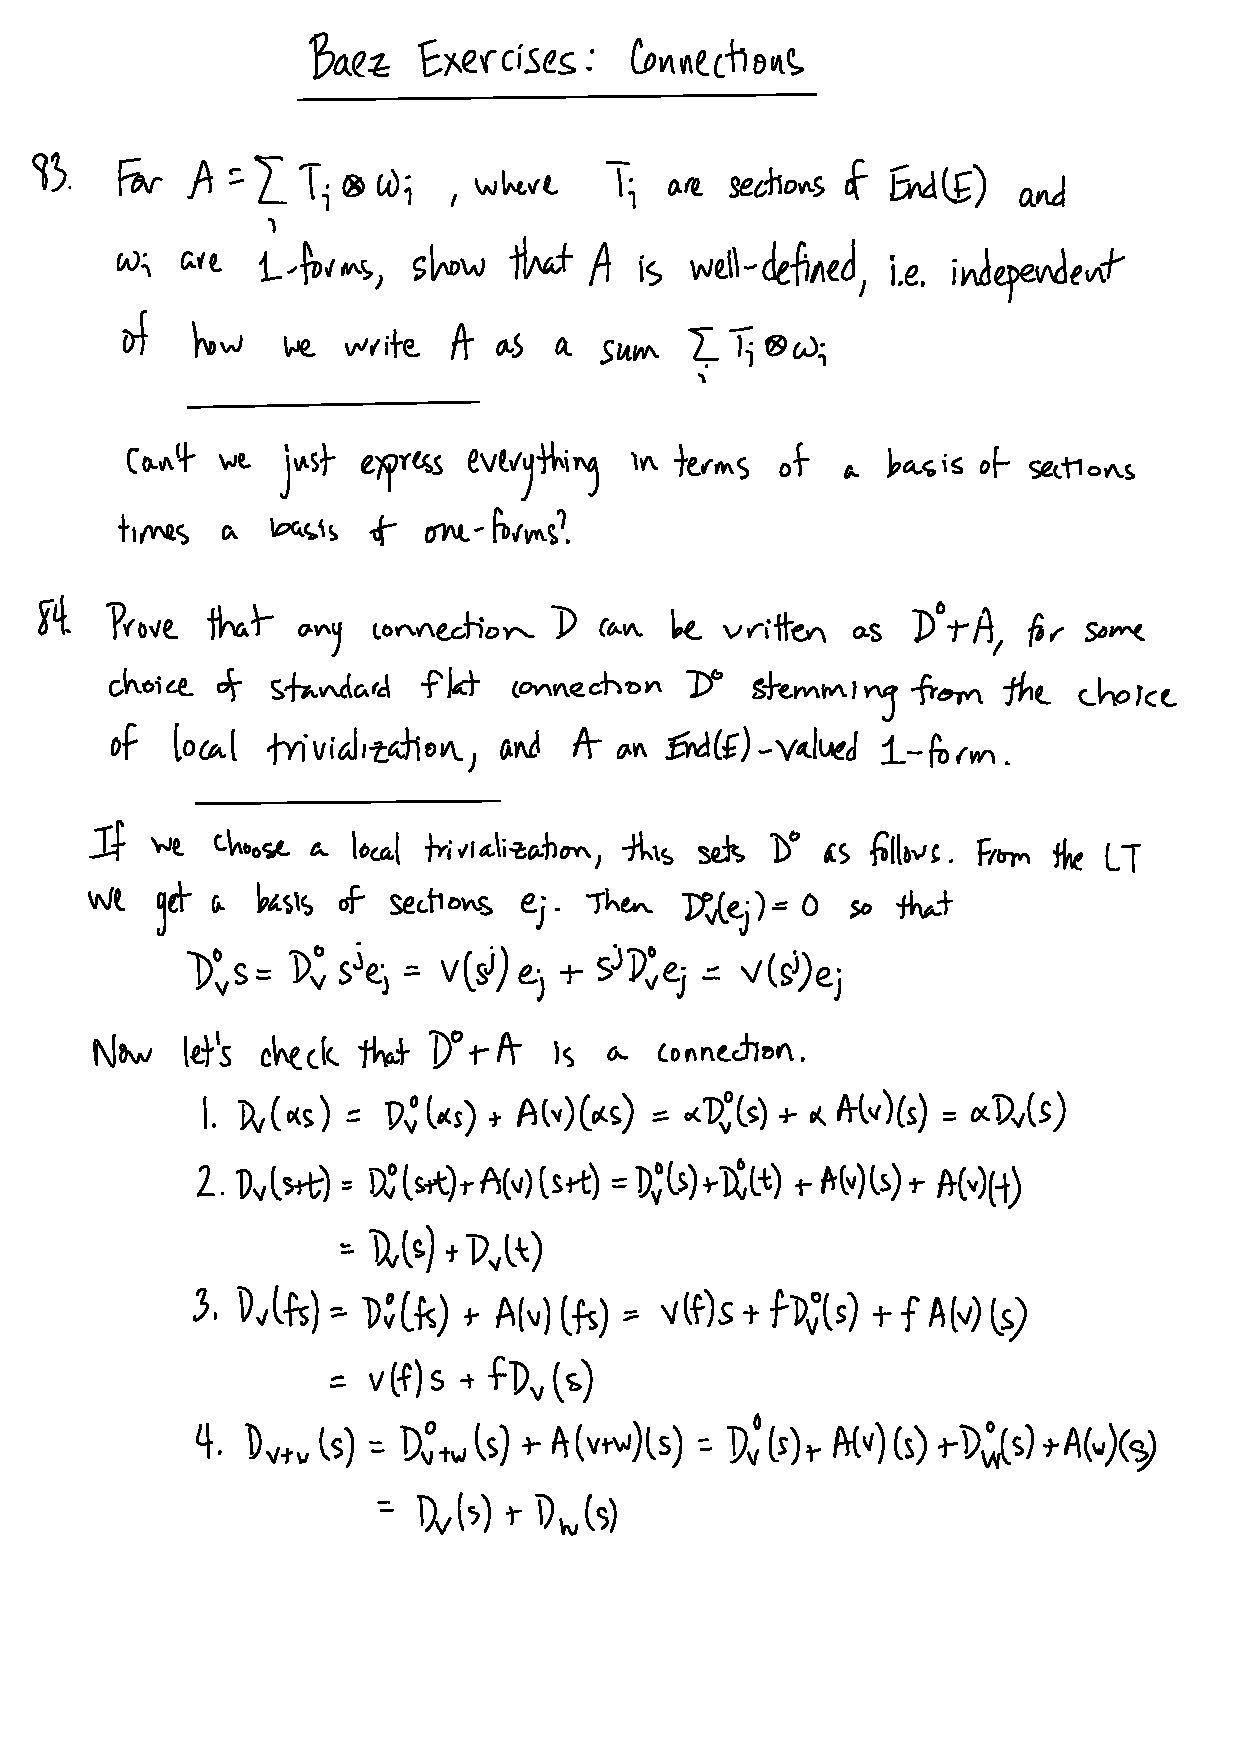
\includepdf[pages=-]{src/gfkg225.pdf}



\setcounter{p}{85}
\begin{p}%86
{Using a local trivialization of $E$ over $U_\alpha\subseteq M$ write the $G$-connection $D$ as the standard flat connection plus a vector potential: $D=D^0+A$. Show that the vector potential $A'$ for $D'$ is given in local coordinates by $$A'_\mu=gA_\mu g^{-1}+g\partial\mu g^{-1}.$$ Show that
since $A_\mu$ lives in $\mathfrak{g}$, so does $A_\mu'$. (Hint: show that if $A_\mu$ lives in $\mathfrak{g}$ and $g\in G$, then $g A_\mu g^{-1}$ lives in $\mathfrak{g}$. Also show that if 
$g\in\mathcal{G}$, $g\partial_\mu g^{-1}$ lives in $\mathfrak{g}$.) Conclude that $D'$ is a $G$-connection.}
\end{p}
{$D'_\mu(s)=gD_\mu(g^{-1}s)=gD_\mu^0(g^{-1}s)+gA_\mu(g^{-1}s)$. The local trivialization 
means that we have chosen a basis of sections $\{e_j\}$ such that $D_\mu^0(s^je_j)=(\partial_\mu s^j)e_j$. The action of $g$ can be represented by $g=\rho(g)^j_k e_j\otimes e^k$ and the corresponding
flat covariant derivative is just $D_\mu^0(g)=(\partial_\mu \rho(g)^j_k)e_j\otimes e^k$. Inserting these expressions into $D'_\mu(s)$ gives 
\begin{align}
D'_\mu(s)&=g D_\mu(g^{-1}s)=gD_\mu^0(g^{-1}s)+gA_\mu(g^{-1}s)\\
&=g\left(\partial_\mu \rho(g^{-1})^k_j s^j\right) e_k+gA_\mu g^{-1}s
=D_\mu^0(s)+g\left(\partial_\mu \rho(g^{-1})^k_j \right)s^j e_k+gA_\mu g^{-1}s\\
&=D_\mu^0(s)+gD_\mu^0(g^{-1})s+gA_\mu g^{-1}s=D_\mu^0(s)+(g\partial_\mu g^{-1})s+gA_\mu g^{-1}s,
\end{align}
where in the last equality we've abuse notation somewhat. Hence the vector potential has changed
according to the prescribed form. For $g\in\mathcal{G}$, $g\partial_\mu g^{-1}$ lives in $\mathfrak{g}$ for the following reason. Really this expression is $\rho(g)^j_\ell \partial_\mu \rho(g^{-1})^{\ell}_k(x^\nu)$ and $\rho(g)(x^\nu)=\exp\left(-c_j(x^\nu)h^j\right)$, where
$h^j$ is a generator set for the Lie algebra $\mathfrak{g}$. Thus, $g\partial_\mu g^{-1}=(\partial_\mu c_j(x^\nu))g h^jg^{-1}$, which is
an element of $\mathfrak{g}$. 
 }

 \begin{p}%87
 \end{p}

 \newpage

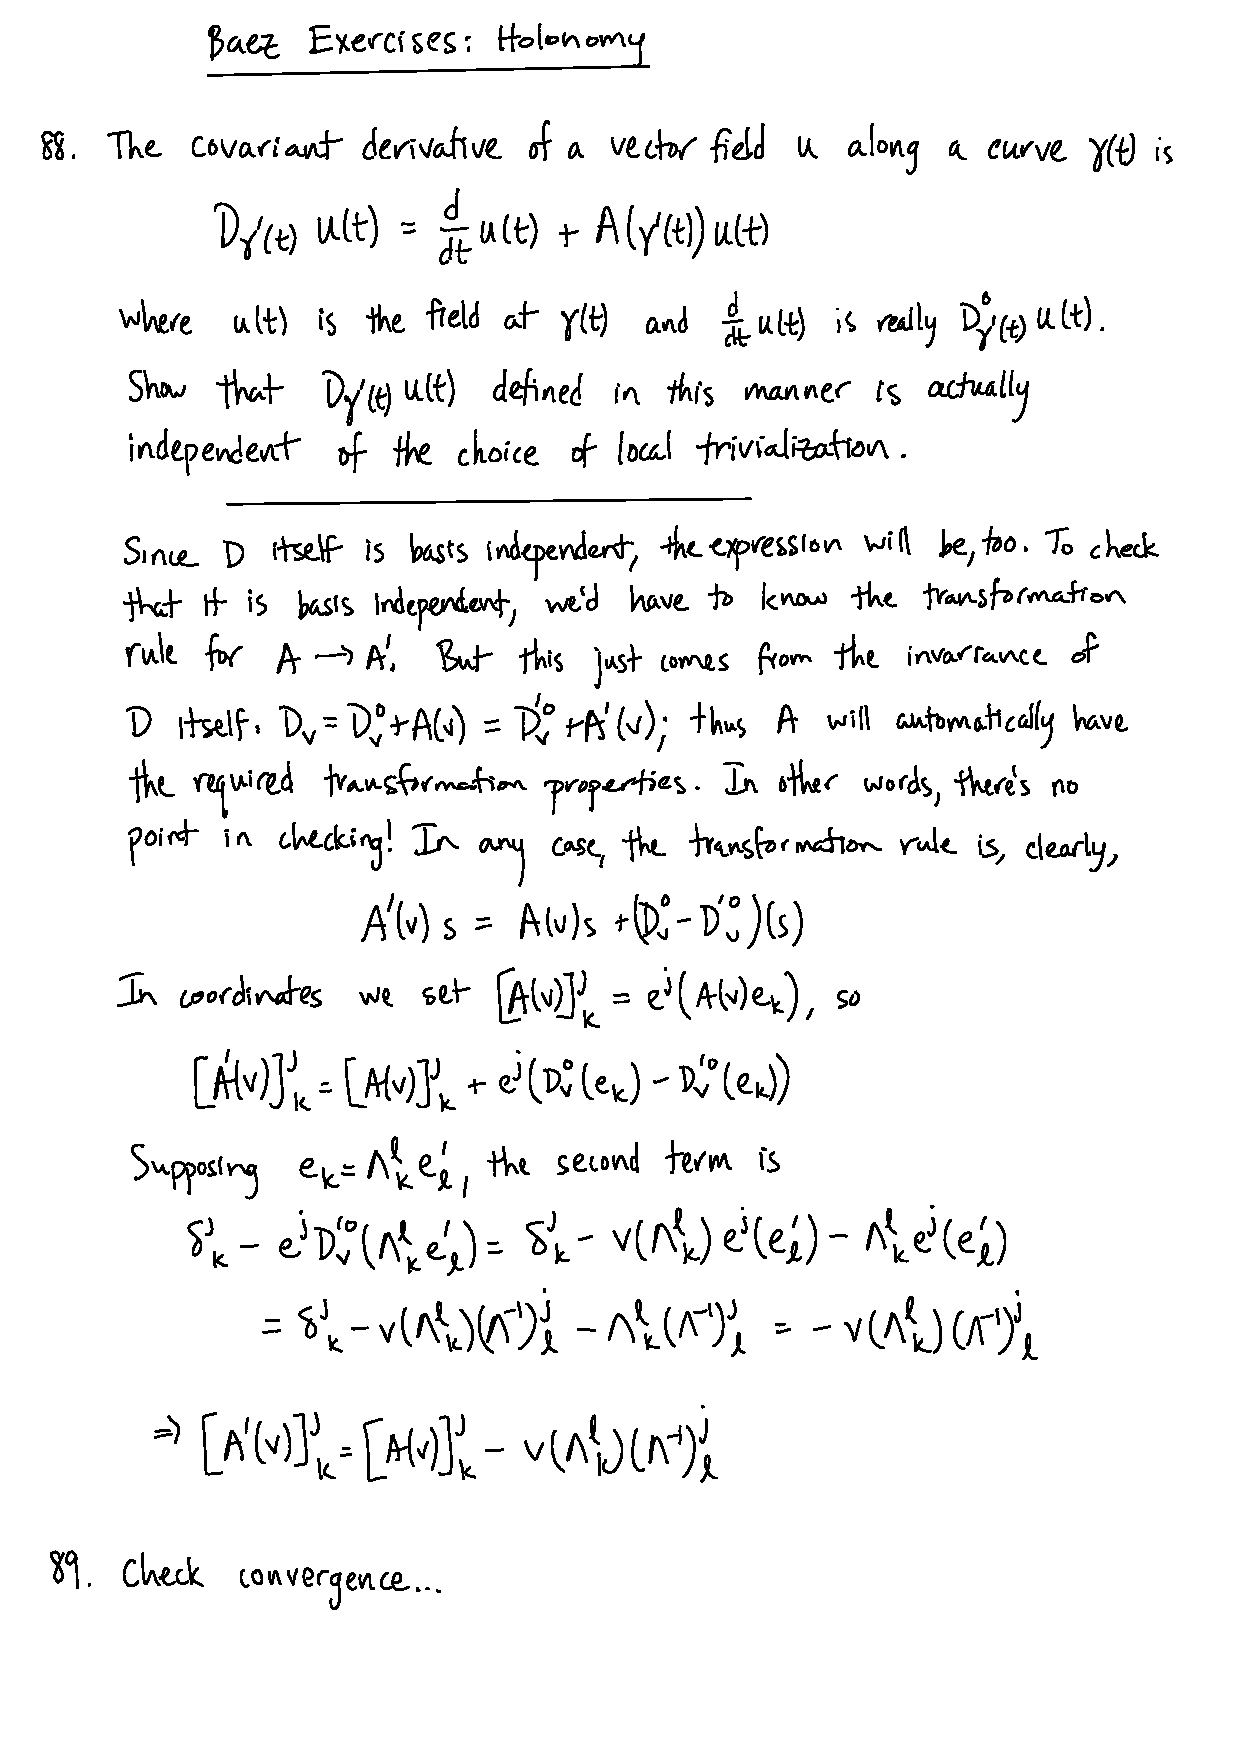
\includepdf[pages=-]{src/gfkg226.pdf}

